\documentclass[10pt,a4paper]{article}
\usepackage[margin=0.80in]{geometry}
\usepackage[T1]{fontenc}
\usepackage[utf8]{inputenc}
\usepackage{lmodern,microtype}
\usepackage{amsmath,amssymb,amsthm,mathtools}
\usepackage{booktabs,tabularx,array,enumitem,xcolor,tikz}
\usepackage{hyperref,fancyhdr}
\usetikzlibrary{arrows.meta,positioning,calc}
\definecolor{navy}{HTML}{143451}
\definecolor{teal}{HTML}{137C80}
\definecolor{grayink}{HTML}{4F5E69}
\definecolor{shade}{HTML}{E9F1F2}
\hypersetup{colorlinks=true,urlcolor=teal,citecolor=teal,linkcolor=navy,pdfauthor={Mohammad Amanlou},pdftitle={REFLEX 8.0: Refutable Certificates without a State Oracle}}
\pagestyle{fancy}\fancyhf{}\fancyhead[L]{\footnotesize\textcolor{grayink}{REFLEX 8.0 | Mathematical research note}}\fancyhead[R]{\footnotesize\textcolor{grayink}{22 November 2026}}\fancyfoot[C]{\thepage}\setlength{\headheight}{13pt}
\setlist[itemize]{leftmargin=1.3em,itemsep=2pt,topsep=2pt}
\setlist[enumerate]{leftmargin=1.3em,itemsep=2pt,topsep=2pt}
\newtheorem{theorem}{Theorem}
\newtheorem{lemma}[theorem]{Lemma}
\newtheorem{proposition}[theorem]{Proposition}
\newtheorem{corollary}[theorem]{Corollary}
\newtheorem{definition}[theorem]{Definition}
\newcommand{\F}{\mathbb F_2}
\newcommand{\Pset}{\mathcal P}
\newcommand{\Hon}{\mathcal H}
\newcommand{\Cert}{\mathsf{Cert}}
\newcommand{\xor}{\mathbin\oplus}
\newcommand{\supp}{\operatorname{supp}}
\begin{document}
\begin{center}
{\footnotesize\textcolor{teal}{EXPLORATORY THEORETICAL MANUSCRIPT --- NOT PEER-REVIEWED}}\\[5pt]
{\LARGE\bfseries\textcolor{navy}{REFLEX 8.0: Refutable Certificates\\[2pt] without a State Oracle}}\\[5pt]
{\normalsize\bfseries The Detection--Correction--Equilibrium Frontier for Delegated Agent Audits}\\[6pt]
{\small Mohammad Amanlou | University of Tehran | 22 November 2026}\\[2pt]
{\footnotesize\textbf{Code and reproducibility:} \url{https://github.com/MohammadAmanlou/REFLEX}}
\end{center}
\vspace{3pt}
\noindent\colorbox{shade}{\parbox{.965\linewidth}{\small\textbf{Research-integrity boundary.} We prove the results below for a \emph{finite binary} principal-labelled measurement model with bounded corrupted owners and authenticated measurements from noncorrupted owners. This note replaces the previous assumption of \emph{detecting who lied} with checkable \emph{counterevidence}. No global truth oracle is used, but local measurement semantics and proof authenticity remain assumptions. The detection--correction gap, evidence-based implementation, optimistic challenges, and robust set-cover concepts have substantial prior art; historical novelty and top-conference readiness are \emph{not} demonstrated.}}
\begin{abstract}
Can a network of self-interested delegated AI agents avoid ratifying false collective decisions without any referee who already knows the correct answer? We study a binary owner-labelled audit graph with arbitrary agent offsets, owner-level Byzantine manipulation, and verifiable cycle-parity counterevidence. We prove an exact three-regime separation: if the minimum owner transversal of decision-sensitive cycles is at most $k$, no transcript-based rule can simultaneously be honest-complete and $k$-sound; if it lies between $k+1$ and $2k$, abstaining sound certification is possible but total recovery is impossible; above $2k$, exact recovery is possible. We then specify a \emph{post-commit refutation game} whose challenge bounties make every subgame-perfect equilibrium free from \emph{false finalized certificates}, conditional on at most $k$ Byzantine principals and bounded honest challengers' outside incentives. In a distributed-evidence extension, robustness depends not only on the graph but on which independently authenticated principal can actually assemble a counterexample; we give an explicit witness-accessibility cut and exact small-instance custody synthesis. Exhaustive synthetic tests verify the predicted regimes and a pure-strategy challenge game. These results sharpen the program, but do not solve unrestricted collusion-proof truth elicitation or independent historical novelty.
\end{abstract}

\section{Why the previous incentive theorem was insufficient}
REFLEX 7.0 obtained an exact forgery-cost frontier and an audit-policy linear program, but its strategic guarantee required independently detecting a principal's manipulation. Such detection is nontrivial when the state to be certified is itself unknown. We replace the demand ``prove this principal lied'' with the narrower, syntactically verifiable demand ``exhibit valid signed measurement receipts whose cyclic parity \emph{contradicts the proposed state}.'' This accepts that \emph{some true decisions may be deferred}; our primary goal is to reject false certainty.

This is not the invention of optimistic fraud proofs, peer mechanisms, or verifiable evidence. Peer-prediction work documents nontruthful equilibria \cite{kong2018,lehmann2025}; evidence-based full implementation has a separate mature theory \cite{banerjee2024,robust2026}; optimistic challenge games have been analyzed for free riding and incentive fragility \cite{incentive2026}; and prior agentic AI work studies strategic auditing \cite{das2026} and contracts under delegation \cite{davoust2020}. Our precise, restricted synthesis is the \emph{owner-labelled detection versus correction threshold together with evidence-custody availability and an explicit equilibrium-safe refutation subgame}. Whether that synthesis is publication-novel needs external theorem-level review.

\section{Binary authority-labelled measurement model}
Let $G=(V,E)$ be a finite \emph{simple undirected graph}. Every vertex $v$ represents a delegated context and an authenticated registry maps it to ultimate principal $\rho(v)\in\Pset$. The unknown state is $h\in\F$. For each edge $e=uv$ there is a stipulated decision sensitivity $b_e\in\F$ and a signed edge receipt:
\begin{equation}\label{eq:measurement}
 y_e=s_u\xor s_v\xor b_eh\xor\eta_e,\quad s_v\in\F.
\end{equation}
Offsets $s$ are unrestricted and can be correlated. A Byzantine set $S\subseteq\Pset$, $|S|\le k$, may manipulate any $y_e$ incident to a context owned by $S$; all other edge measurements must satisfy Eq.~\eqref{eq:measurement} with $\eta_e=0$. A \emph{$b$-odd cycle} $C$ is a simple cycle with $\bigoplus_{e\in C}b_e=1$. The parity $\chi_C(y)=\bigoplus_{e\in C} y_e$ cancels all vertex offsets and equals $h$ on a fully noncorrupted cycle.

\begin{definition}[Principal odd-cycle transversal]
Let $V(S)=\rho^{-1}(S)$. Define
\begin{equation}\label{eq:tau}
 \tau=\min\big\{|S|:G-V(S)\text{ has no $b$-odd simple cycle}\big\}.
\end{equation}
The value is $0$ if $G$ originally has no such cycle; cloning delegates owned by the same authentic principal does not create independent corruption tolerance.
\end{definition}

Let $\Hon_h^{(k)}$ be the \emph{set of all possible complete transcripts} under state $h$, arbitrary offsets, and at most $k$ corrupted principals. The superscript $0$ denotes completely uncorrupted receipts. A transcript-based rule is \emph{honest-complete} if it outputs $h$ for every $y\in\Hon_h^{(0)}$, and \emph{$k$-sound} if it never outputs $1-h$ for any $y\in\Hon_h^{(k)}$. It may abstain ($\bot$).

\section{Three-regime theorem: correct, defer, or impossible}
\begin{lemma}[Two transcript-intersection identities]\label{lem:intersection}
For any integer $k\ge0$,
\begin{align}
 \Hon_0^{(0)}\cap\Hon_1^{(k)}=\varnothing &\iff \tau>k,\label{eq:one}\\
 \Hon_0^{(k)}\cap\Hon_1^{(k)}=\varnothing &\iff \tau>2k.\label{eq:two}
\end{align}
The first identity is symmetric in the states.
\end{lemma}
\begin{proof}
If one transcript has representations in worlds $h=0$ and $h=1$, subtracting the two equations over $\F$ gives $b=D(s_0\xor s_1)\xor\eta_0\xor\eta_1$. Outside the owners corrupted in either representation, the vector $b$ is a coboundary and consequently has parity zero on every surviving cycle. In the first comparison only one corruption set of size at most $k$ appears; in the second, the union of two size-$k$ sets has size at most $2k$. Thus transcript intersection implies a principal transversal with the corresponding cardinality.

Conversely, if removing some owner set $U$ of size at most $k$ (respectively $2k$) destroys every $b$-odd cycle, the restricted $b$ is a coboundary $Dx$ on the remaining graph: this follows by assigning vertex potentials along a spanning forest, with no conflicting signed cycles. Extend $x$ arbitrarily to removed nodes; $b\xor Dx$ is supported on edges incident to $U$. In the first setting assign all discrepancy to one size-$k$ corrupt set. In the second partition $U$ into two sets of cardinality at most $k$ and split the discrepancy coordinatewise between them. This explicitly constructs a shared transcript in the two distinct states.\end{proof}

\begin{theorem}[Exact abstention-aware certification frontier]\label{thm:trichotomy}
For any $k$ the graph belongs to exactly one of the following regimes:
\begin{enumerate}
\item $\tau\le k$: \emph{no transcript-based rule} can be both honest-complete and $k$-sound.
\item $k<\tau\le2k$: an honest-complete, $k$-sound rule exists but \emph{no rule} can always recover $h$ under up to $k$ corruptions.
\item $\tau>2k$: the true state can always be recovered under up to $k$ corruptions.
\end{enumerate}
A rule witnessing the middle regime is
\begin{equation}\label{eq:cert}
 \Cert(y)=\begin{cases}
 h,&\text{if an odd cycle exists and $\chi_C(y)=h$ for every $b$-odd cycle $C$};\\
 \bot,&\text{otherwise.}
 \end{cases}
\end{equation}
\end{theorem}
\begin{proof}
If $\tau\le k$, Lemma~\ref{lem:intersection}'s first identity provides a transcript that is honest under one state but corrupt under the other. Honest completeness forces a false certificate in the latter. If $\tau>k$, every size-$k$ corrupt set leaves at least one fully noncorrupted $b$-odd cycle, whose parity must equal the true state. Thus the opposite state cannot satisfy Eq.~\eqref{eq:cert}. With no corruption, every odd cycle parity equals $h$, so the rule is honest-complete. If $\tau\le2k$, the second identity gives an ambiguous transcript so total recovery is impossible. If $\tau>2k$, the two possible transcript classes are disjoint, allowing a deterministic feasibility decoder that returns the unique state.\end{proof}

\begin{figure}[t]
\centering
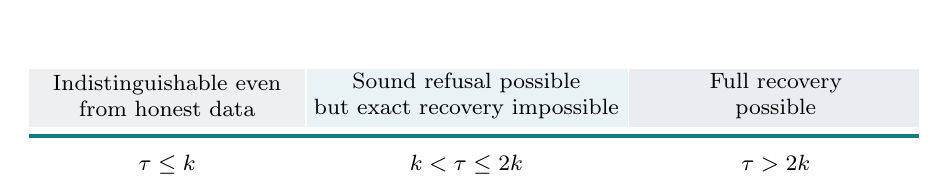
\begin{tikzpicture}[>=Latex, every node/.style={font=\footnotesize}, x=1cm,y=1cm]
\draw[very thick,teal] (0,0)--(11.3,0);
\fill[grayink!10] (0,0.11) rectangle (3.5,0.85);
\fill[teal!9] (3.52,0.11) rectangle (7.6,0.85);
\fill[navy!9] (7.62,0.11) rectangle (11.3,0.85);
\node[align=center] at (1.75,.51){Indistinguishable even\\from honest data};
\node[align=center] at (5.55,.51){Sound refusal possible\\but exact recovery impossible};
\node[align=center] at (9.48,.51){Full recovery\\possible};
\node[anchor=north] at (1.75,-.12){$\tau\le k$};
\node[anchor=north] at (5.55,-.12){$k<\tau\le2k$};
\node[anchor=north] at (9.48,-.12){$\tau>2k$};
\end{tikzpicture}
\caption{The restricted model's detection--correction frontier. The $2k$ gap is intimately related to classical error-detecting versus error-correcting codes; we do not claim that distinction as historically new.}
\end{figure}

\paragraph{Exact example.} With two disjoint $b$-odd triangles, six independently owned vertices, and $k=1$, we have $\tau=2$. No uniformly correct decoder exists: exhaustive enumeration finds 32 full transcripts compatible with \emph{both} states under one owner corruption each. Nevertheless $\Cert$ never certifies the wrong state; an adversary may merely force abstention. Three owner-disjoint triangles give $\tau=3$, crossing the full-correction threshold for $k=1$.

\section{No-state-oracle dispute game and equilibrium safety}
The mechanism is \emph{not} another promise to audit semantic truth later. A proposer publishes a candidate $\hat h$ and commits to available signed edge receipts; the verifier has \emph{no direct oracle for $h$}. In the challenge subgame, eligible principals can reveal an authenticated, accessible $b$-odd cycle $C$ such that $\chi_C(y)\ne\hat h$. The verifier checks only signatures, edge IDs, episode consistency, cycle closure, odd-$b$ parity, and the XOR discrepancy. Every valid challenge cancels certification; invalid challenges pay nothing and may incur their cost. For a valid refutation a designated independent budget pays each distinct authenticated principal a bounty $R_a$ regardless of other valid challengers (no first-mover free-riding). Payments and access are limited to one per registered principal and require the identities to be valid.

A \emph{rational non-Byzantine principal} $a$ has challenge effort cost $c_a$. Let $L_a\ge0$ bound the maximal additional utility they could get from \emph{not} challenging a false claim, including any allowed side compensation, compared with having it rejected; this bound is an explicit assumption, not deduced from the graph. The attacker can control at most $k$ authentic principals, and cannot suppress the authorized disclosures of a non-Byzantine custodian. No unbounded bribery of additional custodians is permitted.

\begin{theorem}[Equilibrium safety with paid counterevidence]\label{thm:eq}
Suppose $\tau>k$, at least one uncompromised rational principal can unilaterally disclose each noncompromised $b$-odd cycle's signed receipts, and for that principal $R_a>c_a+L_a$. Then, after any claimed state, \emph{every Nash equilibrium of the finite challenge subgame} rejects a false claim. Consequently in \emph{every subgame-perfect equilibrium} of any preceding proposal stage, no incorrect state is finalized. Abstention or refusal remains possible, even for a correct claim when some principal is Byzantine.
\end{theorem}
\begin{proof}
For any false candidate and any corruption set $S$ of cardinality at most $k$, $\tau>k$ guarantees a fully uncompromised odd cycle. By the stipulated disclosure access, at least one uncompromised principal $a$ can submit a valid contradicting receipt bundle. If the principal remains silent, the greatest benefit of allowing the false claim to finalize over its rejection is $L_a$. By submitting its valid proof, it earns $R_a-c_a>L_a$, regardless of other challengers because each authenticated valid submission is compensated. Hence silence is strictly dominated in the challenge subgame. In every Nash equilibrium (including mixed equilibria), $a$ challenges with probability one and the false proposal cannot finalize. Backward induction applies to every subgame-perfect equilibrium of the full proposal--challenge game.\end{proof}

\textbf{Crucial scope.} This is \emph{all-equilibria soundness of finalization}, not all-equilibria truthful reporting or guaranteed decision availability. If rewards do not dominate opportunity costs, a no-challenge equilibrium can reappear; if all owners are corrupt or fully bribable, the result does not apply. Fraud-proof bounties and evidence-based implementation are known techniques \cite{banerjee2024,incentive2026}; our theorem is a scoped realization in the owner-labelled cyclic audit model, not proof of a previously unknown universal mechanism.

\section{Who can actually produce a counterexample?}
The previous theorem implicitly presumed custody access. In real delegated-agent systems, a graph can contain mathematically valid evidence that no independent party is allowed to disclose. For every $b$-odd cycle $C$, let $A_C\subseteq\Pset$ be the set of authenticated principal custodians \emph{each able to disclose all necessary receipts alone} (possibly empty). The verifier does not have to possess those receipts before the challenge. A clean and challengeable witness survives a corrupt set $S$ if
\[P(C)\cap S=\emptyset\quad\text{and}\quad A_C\setminus S\ne\emptyset,\]
where $P(C)$ is the set of owners incident to the cycle. Define the \emph{custody-aware witness cut}
\begin{equation}\label{eq:lambda}
 \lambda_A=\min\left\{|S|:\forall C\ b\text{-odd},\ \big(P(C)\cap S\ne\emptyset\ \lor\ A_C\subseteq S\big)\right\}.
\end{equation}

\begin{proposition}[Custody-aware equilibrium-soundness certificate]
If $\lambda_A>k$ and for every surviving accessible witness a non-Byzantine eligible custodian has bounty $R_a>c_a+L_a$, then every subgame-perfect equilibrium avoids false finalization. Moreover $\lambda_A\le\tau$, and when every owner can access every signed receipt, $\lambda_A=\tau$.
\end{proposition}
\begin{proof}
For every corrupt $S$ of size at most $k$, $\lambda_A>k$ leaves a clean odd cycle with at least one honest eligible custodian. Its parity is the true state and its signed receipts refute any opposite proposal. The best-response proof of Theorem~\ref{thm:eq} applies. Every set deleting all odd cycles also deletes all accessible clean cycles, so $\lambda_A\le\tau$. If all owners are eligible custodians (and there is an uncorrupted principal), accessibility adds no cut beyond destroying every odd cycle, giving equality.\end{proof}

\paragraph{Custody synthesis problem.} Available custody grants $g=(C,a)$ have nonnegative costs $c_g$. For $S\subseteq\Pset$, $|S|\le k$, let $g$ \emph{cover} scenario $S$ if $P(C)\cap S=\emptyset$ and $a\notin S$. Then cheapest guaranteed accessible evidence can be chosen by the finite covering integer program
\begin{equation}\label{eq:setcover}
 \min_{x_g\in\{0,1\}}\sum_g c_gx_g\quad\text{s.t.}\quad \sum_{g\text{ covers }S}x_g\ge1\ \ \forall S\subseteq\Pset,\ |S|\le k.
\end{equation}
The construction is an exact reduction to weighted set cover, \emph{not} a novel polynomial-time algorithm. Exhaustive enumeration is implemented for small instances; scalable witness generation and incentive-compatible custody remain future work.

\paragraph{Two-cycle counterexample.} For two disjoint odd triangles with $\tau=2$, a \emph{single} custodian controlling disclosures from both cycles reduces $\lambda_A$ to $1$. Assigning genuinely independent custodians from the separate triangles increases $\lambda_A$ to $2$ without changing the measurement graph. In a four-grant toy library, the cheapest one-Byzantine-safe custody solution costs $2.2$ units; all four costs are synthetic.

\section{Executed computational audit and limitations}
All tests are in \texttt{reflex8\_refutable\_certification.py}, Python standard library only, with deterministic seed. The validation separately enumerates all compatible receipts in both states, principal-compromise subsets, and possible edge tampering masks, rather than assuming the theorem when computing its oracle. An additional two-agent challenge game exhaustively enumerates all pure Nash equilibria. It is a sanity check of the formal claims, not peer review or agent deployment.
\begin{center}\small
\begin{tabularx}{\linewidth}{@{}p{.43\linewidth}X@{}}\toprule
\textbf{Test} & \textbf{Executed result}\\
\midrule
180 random small owner-labelled graphs & All one-sided and two-sided transcript-intersection identities matched $\tau>k$ and $\tau>2k$.\\
Two disjoint signed triangles, $k=1$ & $\tau=2$, 32 ambiguous attacked transcripts, zero false certifications in exhaustive enumeration.\\
Three independent signed triangles, $k=1$ & $\tau=3$: full recovery threshold is satisfied.\\
Shared versus independent custody & $\lambda_A=1$ versus $\lambda_A=2$ with the same underlying graph.\\
Small exact custody optimization & Minimum cost $2.2$ for four synthetic candidate grants.\\
Challenge-game Nash enumeration & Bounty $3$, effort $1$, lost benefit $0.5$: all equilibria challenge. Bounty $1.1$, effort $1$, lost benefit $1$: a no-challenge equilibrium exists.\\
\bottomrule
\end{tabularx}
\end{center}
\noindent\textbf{Limits that still block a top-tier submission.} The binary parity model is stylized; the sensitivity labels $b$ and identity/receipt provenance are assumed correct, not learned; independent signed receipts need not be semantically correct; witnesses might not be affordable or accessible; the bounty game requires a bounded outside benefit and can be exploited via fake contradictory receipts from Byzantine owners (denial of service and bounty farming). Computing all odd cycles is generally expensive. No unrestricted Bayesian game, continuous/noisy signals, stochastic equilibrium selection, multi-principal normative objective, or real LLM agent benchmark is solved.

\section{Highest-value next research question}
The strongest defensible open direction is \emph{incentive-aware placement of independently accessible, semantically valid refutations when every witness's reliability is itself uncertain}. A publishable advance would need a new theorem coupling corruption budgets, constrained evidence custody, bounded rational incentives, and time-uniform error guarantees, with an algorithm that avoids exponential cycle enumeration, and comprehensive comparison to peer prediction, evidence-based implementation, strategic auditing and optimistic verification. It must make substantive predictions that the classical $k$ versus $2k$ coding distinction cannot explain alone.

\textbf{Fit with Professor Michael Rovatsos.} The work asks which institutionally enforceable rules make a community of delegated agents accountable across different human principals, in the spirit of social contracts for noncooperative games \cite{davoust2020}. It should be pitched as a technical question and a four-year research trajectory, not as proof that the professor is supportive, that funding is available, or that a top-tier paper has already been produced.

\section*{Selected related work (primary links)}
\begin{thebibliography}{99}\setlength{\itemsep}{1pt}
\bibitem{davoust2020} A. Davoust and M. Rovatsos. \emph{Social Contracts for Non-Cooperative Games}. AIES 2020. \url{https://www.research.ed.ac.uk/en/publications/social-contracts-for-non-cooperative-games/}.
\bibitem{banerjee2024} S. Banerjee, Y.-C. Chen and Y. Sun. \emph{Direct Implementation with Evidence}. Theoretical Economics 2024. \url{https://onlinelibrary.wiley.com/doi/full/10.3982/TE5015}.
\bibitem{robust2026} \emph{Robust Implementation with Peer Mechanisms and Evidence}. Games and Economic Behavior 2026. \url{https://www.sciencedirect.com/science/article/pii/S0899825625001587}.
\bibitem{kong2018} Y. Kong and G. Schoenebeck. \emph{Equilibrium Selection in Information Elicitation without Verification via Information Monotonicity}. ITCS 2018. \url{https://drops.dagstuhl.de/entities/document/10.4230/LIPIcs.ITCS.2018.13}.
\bibitem{lehmann2025} N. V. Lehmann. \emph{Mechanisms for Belief Elicitation without Ground Truth}. Journal of Economic Surveys 2025. \url{https://onlinelibrary.wiley.com/doi/full/10.1111/joes.70000}.
\bibitem{das2026} S. Das, L. Yu, and H. Zhang. \emph{Optimally Auditing Adversarial Agents}. AAAI 2026. \url{https://ojs.aaai.org/index.php/AAAI/article/download/38722/42684}.
\bibitem{incentive2026} \emph{Incentive Fragility in Optimistic Resolution Mechanisms}. 2026 working paper. \url{https://papers.ssrn.com/sol3/Delivery.cfm/7281058.pdf?abstractid=7281058\&mirid=1}.
\bibitem{lerman2021} G. Lerman and Y. Shi. \emph{Robust Group Synchronization via Cycle-Edge Message Passing}. FoCM 2021. \url{https://link.springer.com/article/10.1007/s10208-021-09532-w}.
\bibitem{cacciamani2024} \emph{Online Information Acquisition: Hiring Multiple Agents}. ICLR 2024. \url{https://proceedings.iclr.cc/paper_files/paper/2024/hash/6358cd0cd6607fdf4870595795eb1710-Abstract-Conference.html}.
\bibitem{sourbut2024} O. Sourbut et al. \emph{Cooperation and Control in Delegation Games}. IJCAI 2024. \url{https://www.ijcai.org/proceedings/2024/26}.
\bibitem{iclr2026} \emph{Truthfulness Despite Weak Supervision: Evaluating and Training LLMs Using Peer Prediction}. ICLR 2026. \url{https://proceedings.iclr.cc/paper_files/paper/2026/hash/650f33fdfaa83f432b9cfa2a2b45d663-Abstract-Conference.html}.
\end{thebibliography}
\end{document}
